\documentclass[12pt,onecolumn,twoside]{article}
\usepackage[T1]{fontenc}
\usepackage[utf8]{inputenc}
\usepackage{amsfonts, amsmath}
% \usepackage{nature}

\usepackage{cell}
\usepackage{natbib}
% The Cell style only works with BibTeX and not BibLaTeX. So load the 'cell' package here, the bib and style file commands in the document at the end, and make sure the cell.bst file is in the same directory as the tex file. Once all of this is in place, compile on the terminal with this sequence: xelatex filename, bibtex filename.aux, xelatex filename, xelatex filename. Atom-latex is a bit unreliable in this regard.

\usepackage[document]{ragged2e} %For non-justified text alignment
\usepackage[margin=0.75in]{geometry}
\usepackage{fontspec}
\setmainfont{Carlito}
\usepackage{hyperref}
\hypersetup{
	colorlinks = true, %Colours links instead of ugly boxes
	urlcolor = blue, %Colour for external hyperlinks
	linkcolor = red, %Colour of internal links
	citecolor = red %Colour of citations
}
%\usepackage{threeparttable}
\usepackage{graphicx}
\usepackage{caption}
\usepackage{subcaption}
% \usepackage{fancyhdr}
% \pagestyle{fancy}
% \fancyhf{}
% \rhead{\thepage}
\makeindex

\usepackage{authblk}
\author{Vibishan B.}
\affil{Department of Biology, Indian Institute of Science Education and Research (IISER), Pune}

\title{Experimental evolution of dispersal and to larval malnutrition in \textit{Drosophila melanogaster}}
\date{\empty}

\begin{document}
	\maketitle
	\section{Introduction}

	\subsection{Dispersal}
	\begin{itemize}
		\item Dispersal is recognised as an important partner in life history evolution.
		\item Dispersal is costly, and is correlated to several phenotypes, physiological and behavioural.
		\item Previous work from the lab has shown that under normal lab conditions, at least components of dispersal can be evolved without any significant cost across many traits (except for dessication and some infections) considered key in life history strategies.
		\item Could it be that the nutritional content of the maintenance food is such that all flies have enough excess energy to allocate for dispersal alongside everything else?
		\item Whole-food dilution is somewhat hairy, and early trials showed that N/3 had the same effect as diluting all components.
	\end{itemize}

	\subsection{Larval malnutrition}
	\begin{itemize}
		\item Our paradigm involves malnutrition at the larval stages => larvae grow in one-third the regular amount of protein.
		\item With or without compensatory feeding, this marks an imbalance in the regular diet of the larvae.
		\item Imbalanced diets have physiological consequences, as shown by the long and storied history of dietary restriction and nutritional geometry in flies.
		\item With these physiological effects as a starting point, it is possible to ask if these proximate mechanisms change reaction norms over the course of adaptation to an imbalanced diet.
	\end{itemize}
	\citep{Ahmad2018}-body size is affected by levels of dietary protein and sugars, foraging stuff from below, and cannibalism. PI3K/Akt has potential connections to many of these processes.
	\citep{Vijendravarma2012}-sitter-rover type polymorphism seen between selected and control populations, under abundant low-quality food. Increase in foraging rate (longer foraging paths, etc) is energy-intensive, and could therefore depend on amount and quality of food. Under crowded conditions, increasing foraging length could lead to better food patches, while uncrowded poor-food environments can possibly not sustain a high-foraging phenotype due to poor food quality. They see their selected populations acting as sitters compared to the unselected ones, and while \textit{for} expression does not follow this expectation, other genetic mechanisms involving \textit{for} are possible.
	\citep{Kolss2009}-evolutionary response to poor food included better egg-to-adult viability, smaller body size and faster development time in poor food, but the plastic response to food quality was mostly the same as the unselected flies. Selected female flies had lower fecundity on normal food compared to unselected ones, but no other trade-offs were found in heat or cold tolerance. Adult survival on normal food is not different between the two, while adults from selected larvae survived worse on poor food; in both these cases, larvae were raised on normal food.
	\section{Methods}
	\subsection{Experimental evolution protocol}
	We begin with four independent large outbred populations (breeding population size ~ 2400) of \textit{Drosophila melanogaster} (DB1-4, short for “Dey Baseline”) in lab which in turn were derived from similar older lines (JB1-4). From each DBi (i $\in$ [1,4]), two populations called VBi (“Vagabond”, subjected to selection for dispersal) and VBCi (not subjected to selection, hence act as controls) were derived. Thus, VB and VBC populations that share the same subscript are related by ancestry. All populations with the same subscript constitute one block. Furthermore, two populations called MDi (“Malnourished Dispersers”, selected for dispersal under malnourished conditions) and MCi (corresponding control for only dispersal) were derived from each VBCi (i є [1,4]). All VB(C) and MD(C) populations are maintained on a 15-day cycle at 25$^{\circ}$C and constant light conditions. For the MD(C) populations, eggs from each new generation are reared on malnourished (N/3 Y) food before the migration assay. Briefly, the set-up consists of three components: source, path and destination. For every generation of MDi, adult flies are introduced into a source container without food or water on the 12th day post-egg collection, and allowed to disperse (currently, a path length of 15m) for 6 hours or till ~50\% of the flies reach the sink, whichever occurs first. MCi populations, at the same time, are kept in source containers under identical conditions for the same duration without undertaking migration.
	\subsection{Dispersal evolution}
	Following 42-43 generations of selection according to the protocol above, assays were carried to determine if any adaptive response has developed in MD compared to MC in response to the dispersal selection regime. All experiments were performed two blocks at a time due to logistic constraints, and after one generation of relaxation to eliminate maternal effects.
	\subsubsection{Dispersal kernel}
	The dispersal kernel is a probability-density function, usually of the distances travelled by a population of dispersers in a given period of time \citep{Clobert2012}. The kernel is a central feature of any dispersal process and can be useful to measure as it carries information about propensity to initiate dispersal, the spatial extent of the population, and potential for change in the distribution.
	The assay setup has a source without food or water, a sink with a small protrusion of the path inside that reduces backflow of flies, and a path of length, 20m. The path is made up of detachable sections of plastic pipes, referred to as bins (twenty 0.5m + ten 1m bins). 12 days post egg collection, ~1000 flies per treatment were introduced into a source (as in Figure 1)  and allowed to disperse for six hours (3 replicates per treatment). After six hours, the bins were sequentially detached and sealed. The flies were heat killed and the number of male and female flies in each bin were counted.

	Two separate components were calculated based on the resulting kernel:
	\[
		\text{Propensity} = \frac{\text{\# of flies outside the source}}{\text{Total \# of flies}}
	\]
	\[
		\text{Ability} = \sum_{i=1}^{y} \frac{x_{i}n_{i}}{n_{i}}
	\]

	where, $y$ is the total number of bins, $n_{i}$ is the number of flies in the $i^{th}$ bin, and $x_{i}$ is the distance of the mind-point of the $i^{th}$ bin from the source.

	\subsubsection{Dry body weight}
	12 days post egg collection, flies were sorted by sex under light C02 anaesthesia, then placed in 1.5mL Eppendorf tubes (20 individuals per tube; 10 replicates per treatment for each sex), and killed by flash freezing. These flies were dried at 60֯C for 72 hrs and body weight was measured to the closest 0.1mg as: (weight of the Eppendorf tubes with flies - weight of empty tubes)/20.
	\subsubsection{Fecundity}
	This assay was conducted 14 days post egg collection in which 55 male-female pairs per treatment were each be kept in a 50 mL Falcon tube (with holes for aeration). The lid contained a small food cup providing a flat surface for oviposition. These set-ups were left undisturbed for 12 hours in a well-lit environment maintained at 25°C. After 12 hrs, the flies were discarded and the number of eggs laid on the food was counted under a microscope.
	\subsubsection{{Locomotor activity (DAM)}}
	Locomotor activity and resting behavior of adult male flies was assayed using the Drosophila Activity Monitoring (DAM2) data collection system (Trikinetics Inc, Waltham, MA) following standard protocols (\cite{Chiu2010}; see also Text S1.2.1). 12 days post egg collection, individual flies were introduced into small glass tubes (length 6.5 cm, diameter 5 mm; 32 replicates per treatment). These tubes were placed in the monitoring apparatus such that two independent perpendicular IR beams pass through the centre of each glass tube. The activity was recorded for 6 h. The activity for a given fly was estimated as the average number of times the fly crossed the IR beam per hour \citep{Chadov2015}. Continuous inactivity for five minutes or more was considered as sleep/rest \citep{Hendricks2000, Chiu2010}.

	\subsection{Dietary modification}
	As noted earlier, the MC populations were derived from VBC and only differ from the latter in the larval diet. An MC-VBC comparison could therefore provide insight into adaptive changes to selection under larval malnutrition. Our approach in this case was a single-generation diet modulation experiment, to look at the response profiles of the two populations to different ratios of dietary protein and carbohydrates.

	All assays were conducted after rearing both MC and VBC on normal food for one generation to minimise any potential non-genetic parental effects. This was done two blocks at a time for logistic reasons. A cornmeal formulation was used for the experimental diets as it allows finer control of protein:carbohydrate ratios in the food through yeast and sugar. Eggs collected from the relaxed populations were reared on cornmeal medium of four different protein:carbohydrate (P:C) concentrations-lowY, eqY, highY and onlyY. Adults eclosing subsequently were assayed for key life-history traits as below.
	\subsubsection{Egg-to-adult viability}
	Exactly 30 eggs were collected per vial for 10 vials per treatment. The number of flies eclosed was counted under $\text{CO}_{2}$ anaesthesia daily from the 8th day post egg collection till the 14th day.
	\subsubsection{Dry body weight}
	12 days post egg collection, flies were sorted by sex under CO2 anaesthesia, then placed in 1.5mL Eppendorf tubes (8-12 individuals per tube; 10 replicates per treatment for each sex), and killed by flash freezing. These flies were dried at 60$^{\circ}$C for 72h. The body weight was calculated to the closest 0.001mg as: $\frac{\text{Weight of the Eppendorf tubes with flies - Weight of empty tubes}}{\text{\# of flies in the tube}}$.
	\subsubsection{Realised fecundity}
	14 days post egg collection, ~40 male-female pairs per treatment were kept in a vial with 6 mL normal banana jaggery food. They were then left to lay eggs for 12h in a well-lit environment maintained at 25$^{\circ}$C. After 12h, the flies were discarded and the vials were maintained under similar conditions. The number of flies eclosed per day was counted every day from the 8th day post egg collection till the 14th day under $\text{CO}_{2}$ anaesthesia.

	\subsection{Statistical analyses}
	Multi-way mixed-model ANOVAs were used for wherever applicable. All ratio data were arcsine-square root transformed and block was considered a random factor wherever it occured in the analysis. Type 3 sums of squares were used in cases of unequal sample sizes between treatments. All analyses were performed on R, using functions from the \texttt{lmerTest} package for fitting mixed-effects models and generating ANOVA tables.

	\section{Results}
	\subsection{Dispersal evolution}
	Figures \ref{fig1} and \ref{fig2} summarise the findings on the evolution of dispersal traits in our fly populations. Both properties of the dispersal kernel measured here show significant responses to the selection regime. MD have higher propensity as well as ability than MC, which means that a larger fraction of the MD population at the source initiate dispersal and on average, travel longer distances than the MC flies. It could also be inferred from these two observations that MD have a larger spatial extent than MC with a flatter kernel curve over the experimental path.
	\begin{figure}
		\centering
		\begin{subfigure}{0.7\textwidth}
			\scalebox{0.5}{\input{fig1a.pdf_tex}}
			\subcaption{\empty}
		\end{subfigure}
		\begin{subfigure}{0.7\textwidth}
			\scalebox{0.5}{\input{fig1b.pdf_tex}}
			\subcaption{\empty}
		\end{subfigure}
		\caption{\label{fig1} Evolution of the dispersal kernel: (a) Propensity was significantly different between the populations ($F_{(1, 5)}$ = 49.4; $p$ = 0.0007), but the sex main effect was insignificant. Propensity values were arcsine-square root transformed for the analysis. (b) Ability was significantly differ between the two populations ($F_{(1, 3)}$ = 42.071; $p$ = 0.0074), but not between the sexes.}
	\end{figure}
	\begin{figure}
		\centering
		\begin{subfigure}{0.49\textwidth}
			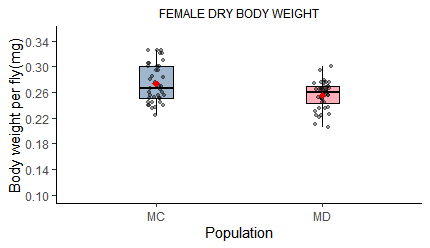
\includegraphics[width=\textwidth, keepaspectratio]{fig1c.png}
			\subcaption{\empty}
		\end{subfigure}
		\begin{subfigure}{0.49\textwidth}
			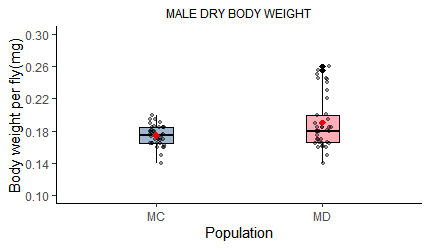
\includegraphics[width=\textwidth, keepaspectratio]{fig1d.png}
			\subcaption{\empty}
		\end{subfigure}\\
		\begin{subfigure}{0.49\textwidth}
			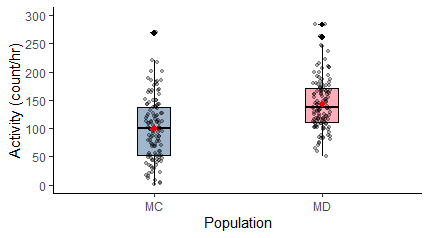
\includegraphics[width=\textwidth, keepaspectratio]{fig1e.png}
			\subcaption{\empty}
		\end{subfigure}
		\begin{subfigure}{0.49\textwidth}
			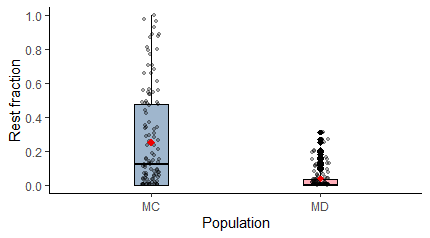
\includegraphics[width=\textwidth, keepaspectratio]{fig1f.png}
			\subcaption{\empty}
		\end{subfigure}
		\begin{subfigure}{0.49\textwidth}
			\centering
			\scalebox{0.6}{\input{fig2.pdf_tex}}
			\subcaption{\empty}
		\end{subfigure}
		\caption{\label{fig2} Trait correlations with evolving the dispersal kernel: Body weight is not significantly different between the two populations in (a) females or (b) males; (c) Average activity count per hour was significantly higher in MD than in MC ($F_{(1, 3)}$ = 17.37; $p$ = 0.025), while (d) fraction of rest bouts was significantly lower in MD ($F_{(1, 3)}$ = 13.48; $p$ = 0.035). Rest fractions were arcsine-square root-transformed for the analysis; (e) Difference in fecundity between the two populations is unclear as the two blocks for which data are available do not show the same trends. Formal statistical analysis is awaiting data from the remaining two blocks.}
	\end{figure}
	\begin{figure}
		\centering
		\scalebox{0.7}{\input{fig3.pdf_tex}}
		\caption{\label{fig3} Response in female body weight to dietary P:C ratios; the populations did not differ from each other although there was a significant main effect on diet ($F_{(1, 3)}$ = 24.23; $p$ = 0.00012).}
	\end{figure}
	\begin{figure}
		\centering
		\begin{subfigure}{\textwidth}
			\scalebox{0.35}{\input{fig4a.pdf_tex}}
			\subcaption{\empty}
		\end{subfigure}
		\begin{subfigure}{\textwidth}
			\scalebox{0.35}{\input{fig4b.pdf_tex}}
			\subcaption{\empty}
		\end{subfigure}
		\caption{\label{fig4} Response in (a) realised fecundity and (b) egg-to-adult survivorship to dietary P:C ratios; the two populations did not differ significantly in either of the traits, but the diet main effect was significant in realised fecundity alone ($F_{(1, 3)}$ = 55.34; $p$ = 8.42*10$^{\text{-6}}$).}
	\end{figure}
	\section{Future outlook}

	\bibliographystyle{cell}
	\bibliography{review}
	% \printbibliography

\end{document}
